%!TeX root=../tese.tex
%("dica" para o editor de texto: este arquivo é parte de um documento maior)
% para saber mais: https://tex.stackexchange.com/q/78101/183146

%% ------------------------------------------------------------------------- %%
\chapter{Modelos de aprendizagem de máquina}
\label{cap:models}

Este capítulo tem como objetivo mostrar como os modelos foram escolhidos e apresentar
métricas nos dados simulados e reais. Os resultados aqui apresentados foram obtidos no 
ambiente do Google Colab, uma vez que que este foi o ambiente escolhido para compartilhar 
os resultados dos nossos experimentos. Por fim, durante a seleção dos modelos apenas os dados 
simulados foram usados, uma vez que ainda não estávamos de posse dos logs reais, portanto 
apenas na última seção deste capítulo mostramos o desempenho do modelo escolhido nos dados reais.


\section{Estrutura dos dados}

No final do capítulo anterior mostrou-se como os arquivos brutos de logs foram transformados
para um formato tabular. As colunas neles contidas podem ser vistas nas tabelas \ref{tab:exemplo_log} e \ref{tab:exemplo_log-2}. 
A seguir é apresentado um dicionário do que significa cada coluna:


\begin{itemize}
    \item ipaddress: o endereço IP do usuário que realizou a requisição.
    \item dateandtime: a data e hora em que a requisição foi realizada.
    \item url: a url requisitada.
    \item statuscode: o código HTTP de retorno.
    \item bytessent: quando bytes foram retornados na requisição.
    \item refferer: se a requisição se originou através de outro website, então o endereço deste 
    website estará nesta coluna. Esse valor é passado através do cabeçalho Refere.
    \item useragent: o agente responsável pela requisição.
    \item malicious: variável indicadora que é 1 se a requisição é maliciosa, 0 caso contrário.
\end{itemize}


\begin{sidewaystable}
\centering

\begin{tabular}{|l|l|l|l|l|l|l|l|}
\hline
ipaddress & dateandtime & navegador & statuscode & bytessent & refferer & malicious & qtd\_query\_params \\ \hline
192.168.0.219 & 13/May/2021:23:38:05 -0400 & Safari & 200 & 2937 & """-""" & 0 & 1 \\ \hline
192.168.0.219 & 13/May/2021:23:38:05 -0400 & Safari & 200 & 2937 & """-""" & 0 & 0 \\ \hline
192.168.0.219 & 13/May/2021:23:38:05 -0400 & Chrome & 200 & 1711 & """-""" & 0 & 0 \\ \hline
192.168.0.219 & 13/May/2021:23:38:05 -0400 & Chrome & 200 & 1675 & """-""" & 0 & 1 \\ \hline
192.168.0.219 & 13/May/2021:23:38:05 -0400 & Chrome & 200 & 1839 & """-""" & 0 & 2 \\ \hline
192.168.0.219 & 13/May/2021:23:38:05 -0400 & Chrome & 200 & 1711 & """-""" & 0 & 1 \\ \hline
192.168.0.219 & 13/May/2021:23:38:05 -0400 & Chrome & 200 & 2306 & """-""" & 0 & 0 \\ \hline
192.168.0.219 & 13/May/2021:23:38:05 -0400 & Chrome & 200 & 1686 & """-""" & 0 & 0 \\ \hline
192.168.0.219 & 13/May/2021:23:38:05 -0400 & Chrome & 200 & 1461 & """-""" & 0 & 1 \\ \hline
\end{tabular}

\caption{Resultado final dos logs - parte 1.\label{tab:exemplo_log}}

\end{sidewaystable}


\begin{sidewaystable}
    \centering
    
    \begin{tabular}{|l|l|l|}
    \hline
    url\_sem\_query & url & useragent \\ \hline
    /index.php & /index.php?extraParam=CwDK... & "Mozilla/5.0 (Macintosh; Intel Mac OS X 10\_9\_3)..." \\ \hline
    /index.php & /index.php & "Mozilla/5.0 (Macintosh; U; Intel Mac OS X 10\_6\_5; ar)..." \\ \hline
    /vulnerabilities/sqli\_blind/ & /vulnerabilities/sqli\_blind/ & "Mozilla/5.0 (Macintosh; Intel Mac OS X 10\_10\_1)..." \\ \hline
    /vulnerabilities/sqli/ & /vulnerabilities/sqli/?extraParam=DfoQ... & "Mozilla/5.0 (Macintosh; Intel Mac OS X 10\_8\_3)..." \\ \hline
    /vulnerabilities/xss\_d/ & /vulnerabilities/xss\_d/?extraParam=QDIa...\&extraParam2=bBj... & "Mozilla/5.0 (Windows NT 10.0; Win64; x64)..." \\ \hline
    /vulnerabilities/sqli\_blind/ & /vulnerabilities/sqli\_blind/?extraParam=Sodj... & "Mozilla/5.0 (Macintosh; Intel Mac OS X 10\_9\_2)..." \\ \hline
    /about.php & /about.php & "Mozilla/5.0 (Windows NT 6.2; WOW64)..." \\ \hline
    /vulnerabilities/xss\_r/ & /vulnerabilities/xss\_r/ & "Mozilla/5.0 (Windows NT 5.1)..." \\ \hline
    /vulnerabilities/weak\_id/ & /vulnerabilities/weak\_id/?extraParam=isBe... & "Mozilla/5.0 (Macintosh; Intel Mac OS X 10\_9\_3)..." \\ \hline
    \end{tabular}
    
    \caption{Resultado final dos logs - parte 2.\label{tab:exemplo_log-2}}
    
\end{sidewaystable}

De posse dessas colunas que estão nos logs, mais 3 colunas foram criadas:

\begin{itemize}
    \item url\_sem\_query: armazena a url requisitada sem o paramêtros de consulta.
    \item qtd\_query\_params: quantidade de parâmetros encontrados na query.
    \item navegador: armazena apenas o nome do navegador presente na coluna useragent.
\end{itemize}


\section{Preparação dos dados}

Durante o treino/validação de todos os modelos deste capítulo, o conjunto de dados original foi dividido 
em treino e teste, como explicado a seguir:

\begin{itemize}
    \item treino: dados que serão usados para treinar o modelo.
    \item teste: dados não presentes no treino, com o objetivo de verificar se o modelo está generalizando bem.
\end{itemize}

Outro ponto de atenção necessário é manter o desbalancemento da variável resposta nos 
conjuntos acima, dado que há mais requisições maliciosas do que não maliciosas. 

Por fim, dados categóricos foram transformados em números usando a técnica de OneHotEncode. Este e o item
anterior foram feitos com o auxílio dos utilitários de pré-processamento de dados do scikit-learn e do Apache Spark.

\section{Modelo base}

O modelo de florestas aleatórias foi escolhido como modelo base. Para avaliar o modelo, as colunas 
abaixo foram escolhidas de maneira árbitrária, ja que neste ponto queríamos saber se modelos de 
árvores resolveriam nosso problema.

\begin{itemize}
    \item statuscode
    \item navegador
    \item qtd\_query\_params
    \item bytessent
\end{itemize}


Com este modelo e as colunas mencionadas conseguimos uma acurácia de 1 nos dados de teste. Surprendente, pois 
não esperávamos esse resultado na primeira tentativa, dado que se trata de um modelo base, logo suspeitamos 
que o modelo estava sobre ajustado nos dados. 

Para ter uma intuição melhor de como o modelo estava realizando a classificação, optamos por experimentar 
o modelo de árvore de decisão, dado que depurá-lo é possível.

\section{Depurando o modelo - árvore de decisão}

As mesmas colunas da seção anterior foram usadas para treinar uma árvore de decisão, e novamente
o modelo teve uma acurácia de 1 nos dados de treino e teste. 

Para entender como a classificação está sendo realizada, exibimos a árvore final na Figura \ref{fig:primeira_arvore}. Nesse sentido, 
como os dados passaram por um pré-processamento de OneHotEncoder vale mencionar o que significa cada índice em X:

\begin{itemize}
    \item X[0] e X[1]: é a coluna statuscode.
    \item X[3] até X[9]: indicam o navegador que foi utilizado.
    \item X[10]: é a coluna qtd\_query\_params
    \item X[11]: é a coluna bytessent
\end{itemize}

\begin{figure}
    \centering
    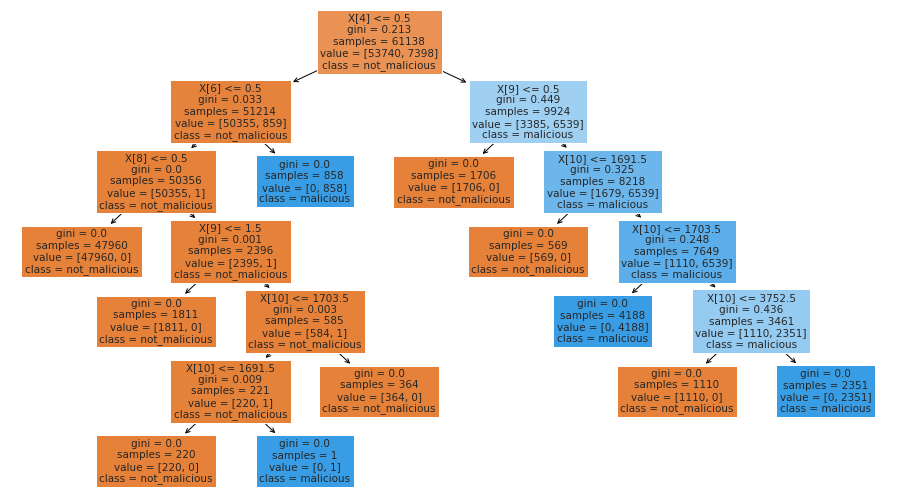
\includegraphics[width=.9\textwidth]{figuras/primeira-arvore.png}
    \caption{Primeira árvore de decisão. Os nós laranjas representam a classe not\_malicious 
    e os azuis a classe malicious. Quanto mais escurto o nó, menor a probabilidade de erro 
    na classificação. \label{fig:primeira_arvore}}    
\end{figure}

Vemos que a árvore está usando majoritariamente os dados da coluna navegador 
para realizar a classifição, o que não faz sentido, uma vez que esse dado foi simulado e o 
navegador não tem nenhuma relação com os ataques. Então removemos essa coluna da entrada 
e o resultado está na Figura \ref{fig:segunda_arvore}.


\begin{figure}
    \centering
    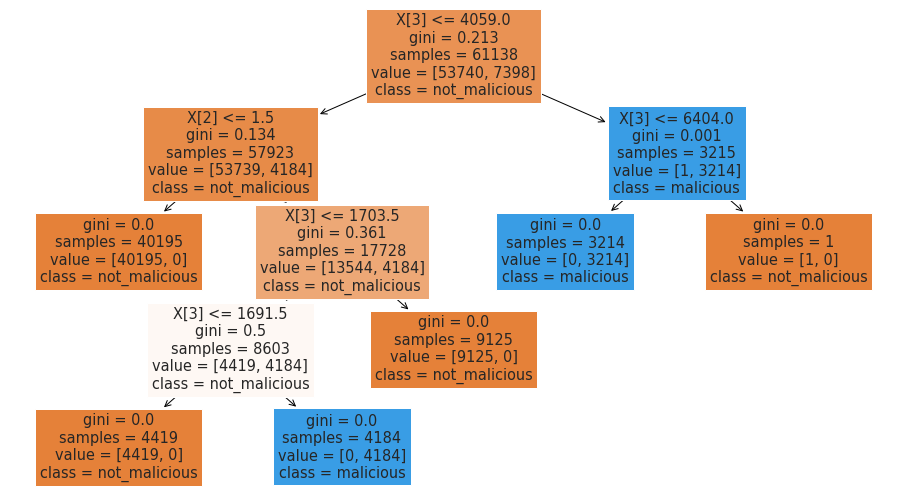
\includegraphics[width=.9\textwidth]{figuras/segunda_arvore.png}
    \caption{Segunda árvore de decisão. Os nós laranjas representam a classe not\_malicious 
    e os azuis a classe malicious. Quanto mais escurto o nó, menor a probabilidade de erro 
    na classificação. \label{fig:segunda_arvore}}    
\end{figure}

Esta versão já nos pareceu mais sólida pois ela utiliza a quantidade de parâmetros na requisição 
e a quantidade de bytes enviados para o cliente, o que está relacionado com os ataques. Além disso,
também atingiu uma acurácia de 1.

\section{Escolha do modelo e considerações}

Dado o que foi apresentado nas seções anteriores, somado aos resultados encontrados no capítulo 2, escolhemos o modelo de árvore de decisão com as colunas
abaixo para realizar os experimentos e valida-lo em dados reais. 

\begin{itemize}
    \item statuscode
    \item qtd\_query\_params
    \item bytessent
\end{itemize}

Outros modelos mais complexos, como redes neurais ou xgboost, não foram considerados pois o 
objetivo deste trabalho é usar o modelo em computadores onde os recursos, como memória e 
disco, são limitados portanto favorecendo modelos mais simples como o escolhido.

Também vale notar que características dos logs específicas a ataques XSS e SQL Injection, como 
verificar a existência de uma consulta SQL na url, não foram criadas pois as colunas padrões 
do log foram suficientes para conseguir uma acurácia considerada boa.

\section{Testes em dados reais}

De posse dos dados reais mencionados na Seção 4.2.2, executamos o modelo escolhido neles e atingimos 
uma acurácia de aproximadamente 0.93 no conjunto de teste. Portanto, definitivamente
seguimos com ele nos experimentos.
